\documentclass{article}

\usepackage[final]{nips_2017}

\usepackage[utf8]{inputenc} % allow utf-8 input
\usepackage[T1]{fontenc}    % use 8-bit T1 fonts
\usepackage{hyperref}       % hyperlinks
\usepackage{url}            % simple URL typesetting
\usepackage{booktabs}       % professional-quality tables
\usepackage{amsfonts}       % blackboard math symbols
\usepackage{nicefrac}       % compact symbols for 1/2, etc.
\usepackage{microtype}      % microtypography
\usepackage{graphicx}
\usepackage{amsmath}
\usepackage{amssymb}
\usepackage{listings}
\usepackage{courier}
\lstset{basicstyle=\ttfamily\footnotesize,breaklines=true}
\title{CSE 253 Programming Assignment 2 -- Multilayers Back-propagation Neural Networks}

\author{
  Fanjin Zeng \\
  Computer Science and Engineering\\
  University of Califorina, San Diego\\
  \texttt{f1zeng@ucsd.edu} \\
   \And
   Xinyue Ou \\
   Computer Science and Engineering\\
   University of Califorina, San Diego \\
   \texttt{x1ou@ucsd.edu} \\
}

\begin{document}

\maketitle
\begin{abstract}
	In this assignment, we design a neural network to classify digits from the mnist dataset. The neural net with one hidden layer of 64 units attain a testing accuracy of 96.96\% after applying "the tricks of the trade." A double layer network with 300 hidden for the first and 100 hidden for the second rewrites the accuracy to be 97.79\%. A network with one layer of 1024 units attains an accuracy of 98.28\%.
\end{abstract}
\section{Classification}
\subsection{}
\subsection{}
\subsection{}
\subsection{}

\newpage
\section{Adding the "Tricks of the Trade"}
\subsection{}
\subsection{}
\subsection{Weight Initialization}
Our code actually starts with this trick. It initializes the weights to be a normal distribution with 0 mean and unit deviation. What's different is that we employ fan-in factor this time. Before the test accuracy is 0.9656 and after that it is 0.9679. It improves a little bit, but not help that much.
\subsection{Momentum}
Momentum is a good way to speed up the training. We compare the difference between the original gradient descent, the one with momentum and the one with Adam optimizer.

\begin{figure}[h]
	\begin{minipage}{0.3\textwidth}
	\centering
	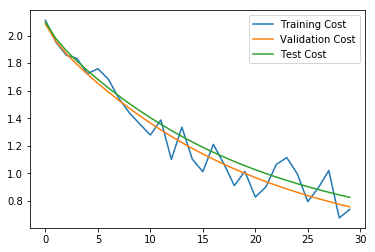
\includegraphics[width=\textwidth]{pics/loss_original.png}
	\caption{Loss function over training epoch. Original gradient descent}
	\end{minipage}\hfill
	\begin{minipage}{0.3\textwidth}
	\centering
	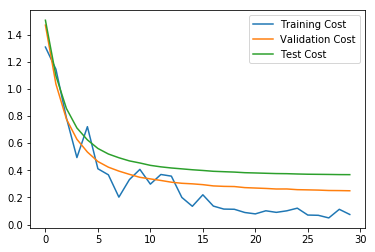
\includegraphics[width=\textwidth]{pics/loss_momentum.png}
	\caption{Loss function over training epoch. Gradient descent with momentum}
	\end{minipage}\hfill
	\begin{minipage}{0.3\textwidth}
	\centering
	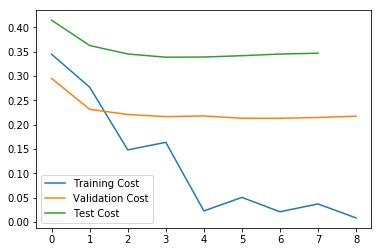
\includegraphics[width=\textwidth]{pics/loss_adam.png}
	\caption{Loss function over training epoch. Adam optimizer}
	\end{minipage}
\end{figure}

The original gradient descent takes 300 epochs of training and arrives at 0.73 loss at the 300th epoch. The gradient descent with momentum also reaches 0.73 loss, but it arrives at the value that is very close to it at the 200th epoch. The Adam optimizer is even faster, it reaches 0.03 at the 80th epoch, and then early stops.


\newpage
\section{Experiment with Network Topology}
\subsection{Double Hidden Units}
When doubling the number of hidden units, i.e., training with 128 neural in the hidden layers, we achieve a test rate of 96.5\%, which is not that different from the one with 64 layers. The tricky part is, when we keep increases the number of hidden layer, the accuracy actually went up quite significantly, reaching more than 98\%.
\begin{figure}[h]
\centering
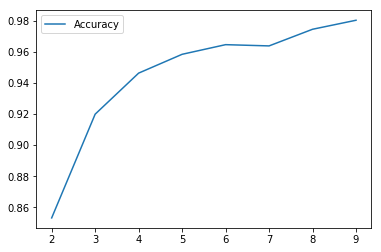
\includegraphics[width=0.5\textwidth]{pics/acc_hidden.png}
\caption{Testing accuracy vs hidden unit number in log scale}
\end{figure}
If the number of the hidden units is too small, the accuracy goes down, but higher number of hidden units significantly increases the training period.

\subsection{Double Hidden Layers}
We use a network with first layer having 48 units and the second one having 16. The testing accuracy of it is 96.21\%. It does not have significant improvement on the accuracy.
\begin{figure}[h]
	\begin{minipage}{0.48\textwidth}
	\centering
	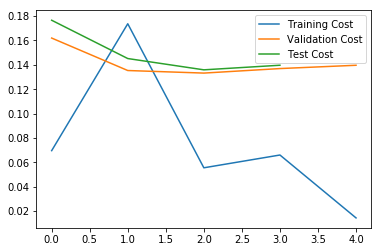
\includegraphics[width=\textwidth]{pics/loss_double.png}
	\caption{Loss function over training epoch, with first hidden layer having 48 units and the second having 16}
	\end{minipage}\hfill
	\begin{minipage}{0.48\textwidth}
	\centering
	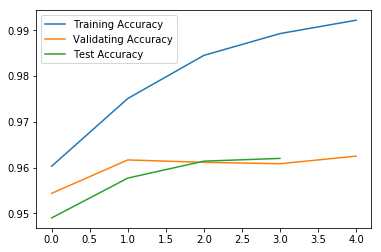
\includegraphics[width=\textwidth]{pics/acc_double.png}
	\caption{Loss function over training epoch, with first hidden layer having 48 units and the second having 16}
	\end{minipage}
\end{figure}

Another network we use is a network with 300 hidden units for the first hidden layer and 100 hidden units for the second hidden layer. It gets an accuracy of 97.79\%
\begin{figure}[h]
	\begin{minipage}{0.48\textwidth}
	\centering
	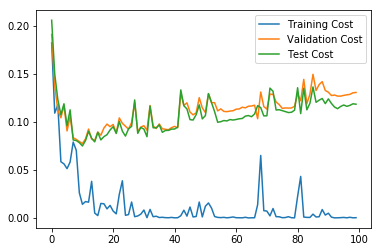
\includegraphics[width=\textwidth]{pics/loss_300_100.png}
	\caption{Loss function over training epoch, with first hidden layer having 300 units and the second having 100}
	\end{minipage}\hfill
	\begin{minipage}{0.48\textwidth}
	\centering
	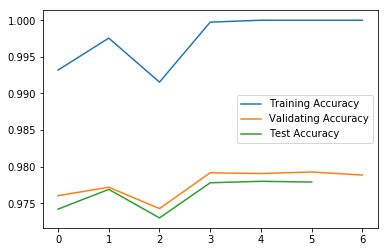
\includegraphics[width=\textwidth]{pics/acc_300_100.png}
	\caption{Loss function over training epoch, with first hidden layer having 300 units and the second having 100}
	\end{minipage}
\end{figure}

\subsection{Extra: Adam Optimizer}
We use adam optimizer for updating parameters, which usually helps to get faster convergence. The result has been mentioned above.  


\newpage
\section{Summary}
To conclude, in this assignment, we build a neural networks to to discriminate digits of ten categories. Starting with a accuracy of 95\%, we improve the accuracy by using proper weight initialization, activation function, and momentum method to accelerate the training. We also explore different network structure to find the best result. 

The best result we achieve is 98.28\% with 1024 hidden units during the experiment playing with the number of hidden units.  With Adam optimizer it learns quickly for about 60 epochs.
Except for this exceptionally large network, we have a two-hidden-layer network with 300 hidden units and 100 units respectively which achieve a result of 97.79\% of testing accuracy.

From this assignment, we learn neural network implementation and apply some tricks of trade to it. While proper preprocessing and weight initialization can improve the accuracy a little bit, momentum can increase the learning speed. Also increasing the number of hidden units can increase the accuracy rate quite a lot while deepening the network with the same number of weight parameter does not pose a significant improvement.
\section{Contributions}
Fanjin Zeng is in charge of the derivation and the implementation of back propagation. He introduces adam optimizer to the model that significantly improves the performance. 

Xinyue Ou is in charged of training the model using different network structures and improving the performance.


\section{References}
[1] Bishop, C. M., {\it Neural networks for pattern recognition}, Oxford: Oxford University Press, 2013.

\end{document}